\documentclass[12pt]{article}

\usepackage{xspace}
\usepackage{lineno}
\usepackage{setspace}
\usepackage{graphicx}
\usepackage{subfigure}
\usepackage{float}
\usepackage{color}
\usepackage{caption}
\usepackage[margin=1in]{geometry}
\usepackage{natbib}
\usepackage{amsmath}


\begin{document}
\doublespacing
\linenumbers

\newcommand{\kluyveri}{\textit{L. kluyveri}\xspace}
\newcommand{\dubl}{\textit{C. dubliniensis}\xspace}
\newcommand{\gossypii}{\textit{E. gossypii}\xspace}


\noindent RH: LANDERER ET AL.--- Intragenomic variation in codon usage
% put in your own RH (running head)
% for POVs the RH is always POINT OF VIEW
\bigskip
\medskip
\begin{center}

% Insert your title:
\noindent{\Large \bf Differences in Codon Usage Bias between genomic regions in the yeast \textit{Lachancea kluyveri}.}
\bigskip

% We don't use a special title page; the author information is entered
% like any other text.

% FOOTNOTES: We don't allow them in the manuscript, except in
% tables. Don't include any footnotes in the text.


\noindent{C\textsc{EDRIC} ~{L\textsc{ANDERER}}$^{1,2,*}$,
R\textsc{USSELL} {Z\textsc{ARETZKI}}$^{3}$,
\textsc{AND}
M\textsc{ICHAEL} A.~{G\textsc{ILCHRIST}}$^{1,2}$}

\end{center}

\vfill

{\small
\noindent$^{1}$Department of Ecology \& Evolutionary Biology, University of Tennessee, Knoxville, TN 37996-1610\\
\noindent$^{2}$National Institute for Mathematical and Biological Synthesis, Knoxville, TN 37996-3410\\
\noindent$^{3}$Department of Business Analytics \& Statistics, Knoxville, TN ~ 37996-0532 \\
\noindent$^{*}$Corresponding author. E-mail:~cedric.landerer@gmail.com
}

\vfill
\centerline{Version dated: \today}
\vfill
\newpage


\begin{abstract}
Large efforts have been made to develop and explore models to understand intra-genomic variation in codon usage bias (CUB) and the contributions of mutation and selection to its evolution.
Comparative studies have been undertaken to further our understanding of variation in codon usage between species.
However, limited efforts have been made to understand how CUB is affected by, and in return effects hybridization or introgression events between species with potentially large differences in CUB. 
In this study, we explore the CUB of \textit{Lachancea kluyveri} which has experienced a large introgression covering the whole left arm of chromosome C, affecting about 10\% of all genes.
The \kluyveri genome provides insights about the adaptation of introgressed regions to a novel genomic environment, with potentially large differences in selection for translation efficiency due to factors like tRNA availability, effective population size, or differences in mutation environment.

We analyzed the CUB of the endogenous \kluyveri genome and compared it to the CUB of the exogenous, introgressed, region while separating the effects of mutation bias and selection for translation efficiency on CUB.
Our results show distinct CUB between the endogenous and exogenous regions of the \kluyveri genome and we show that this differences can be mostly attributed to differences in mutation bias.

The introgression into the \kluyveri genome is of additional interest as the source has not yet been identified.
We explored if the understanding about CUB evolution gained in this study can be used to identify possible candidates for the origin of the introgression experienced by \kluyveri.
The estimation of CUB and its separation into contributions of mutation and selection across a variety of yeasts allowed us to identify two candidates, \textit{Candida dubliniensis} and \textit{Eremothecium gossypii}, for the origin of the exogenous genes.
We used orthogonal information on synteny to validate the candidates we obtained using CUB.
\end{abstract}	



\section*{Outline}

\subsection*{Introduction}

\begin{itemize}
	\item CUB results from mutation, selection, and drift.
	\item Most studies assume that all genes have evolved in the same environment for mutation, selection and drift with differing impact.
	\begin{itemize}
		\item This assumptions can be violated for multiple reasons, like introgression/horizontal gene transfer (HGT), population bottlenecks, etc.
	\end{itemize}
	 \item Genes with different signatures of CUB environments have previously only been studied in bacteria where HGT is common.
	\begin{itemize}
		\item HGT only transfers small number of genes, probably with little to no impact on overall CUB.
		%\item However, exogenous material can accumulate if HGT is frequent \citep{lawrence1997}.
		%\item Previous studies have shown that genes with similar CUB are more likely to be transferred, potentially mitigating effects of accumulation \citep{tuller2011} (we observe only small effects in e.coli).
		\item Hybridization/Introgression between species with different CUB environments should have a larger impact on CUB due to the amount of material transferred, possibly affecting the outcome of a study if ignored. 
	\end{itemize}
	\item In this study, we look at \kluyveri which experienced an introgression, clearly marked by elevated GC content ($13 \%$) (three key results).
	\begin{itemize}
		%\item \kluyveri has experienced a recent ($55.5e6$ generations) large scale introgression \citep{friedrich2015}, clearly marked by elevated GC-content \citep{payen2009}.
		\item CUB differs between the introgressed exogenous region and the endogenous region.
		\begin{itemize}
			%\item We find differences in CUB between the two regions.
			\item Taking this difference into account, we can increase our ability to extract biological information (like predicting gene expression).
			\item We observe greater difference between the regions in mutation bias than in selection for translation inefficiency.
			%\begin{itemize}
			%	\item We expect that the signature of the origin environment would have a faster decaying selection component than mutation component.
			%	\item We, however find evidence that the donor species of the exogenous environment has had a similar selective environment for translation efficiency.
			%\end{itemize}
			%\item Note: Figure \ref{fig:cub_all_aa} shows the CUB if we ignore the introgression (dotted), and for the endogenous (solid) and exogenous (dashed) respectively.
		\end{itemize}
		\item We compares CUB parameters ($\Delta M$ and $\Delta \eta$) inferred from the exogenous genes to $45$ other yeast species and identified \gossypii and \dubl as potential origin of the exogenous genes.  
		\begin{itemize}
			%\item We analyzed CUB for several yeasts and found several species with similar selection for translation efficiency, and a few with similar mutation bias, but only two with high agreement in both (gossypii and dubliensis, Figure \ref{fig:corr_all_species}).
			%\item We validated our findings with orthogonal information from synteny where we analyzed a subset of our initial yeast set closely related to our two candidates and \kluyveri.
			\item Validation of our inference with synteny revealed that \dubl does not show any synteny, leaving \gossypii as potential origin.
			%\item We found several closely related species with syntenious regions, but only one species that also showed agreement in CUB allowing us to exclude dubliensis since it does not show any synteny with \kluyveri (Figure \ref{fig:synteny_species} right).
		\end{itemize}
		\item Assuming \gossypii as origin for the exogenous region, we estimated a time since introgression from our estimates of mutation bias ($5e8$ generations).
		%\begin{itemize}
%			\item Based on the two codon amino acids we estimated a time since introgression on the order of $10e8$
%			\item Assuming one to eight generations per day, we are finding an introgression age between 110k and 890k years, which overlaps with a previous estimate \citep{friedrich2015}.
			%\item The exogenous CUB signature is expect to decay to one percent of the endogenous CUB signature within $5e9$ generation.  
		%\end{itemize}
	\end{itemize}
\end{itemize}

\subsection*{Results}

\begin{itemize}
	\item We compared model fits of CUB for \kluyveri. % with a fit where we allowed CUB to vary between the endogenous and exogenous region.
	\begin{itemize}
		\item Model selection by AIC favored varying CUB between the endogenous and exogenous region of the \kluyveri genome.
		\item Comparison of predicted protein synthesis $\phi$ of both fits with empirical estimates showed that varying CUB improved our ability to predict $\phi$ ($\rho$: $0.59$ vs $0.69$) (Figure \ref{fig:phi_corr_two_cond}).
		%\item We also observed a decrease of the variation in estimated $\phi$ in the homogeneous model fit.
	\end{itemize}
	\item Comparison of posterior estimate of codon specific parameters ($\Delta M$ and $\Delta \eta$) between regions shows a negative correlation for $\Delta M$ and a positive correlation for $\Delta \eta$ (Figure  \ref{fig:csp_comp}).
	\begin{itemize}
		%\item We find a negative correlation of $\Delta M$ between the exogenous and endogenous regions, indicating that both environments have evolved in different mutation environments.
		%\item We find that only 14 out of 40 $\Delta M$ parameters show the same sign, meaning that only $35 \%$ of $\Delta M$ agreed between regions (Figure \ref{fig:csp_comp}). 
		\item Only two amino acids (A,F) favor the same codon by mutation in the two regions.
		%\item Estimates of selection for translation inefficiency ($\Delta \eta$) showed a positive correlation, indicating a similar selection environment between donor and \kluyveri (Figure \ref{fig:csp_comp}).
		\item Nine amino acids share a preferred codon between endogenous and exogenous region%, the other 11 have $\Delta \eta$ close to zero in one or both regions (signature of transition?).
		%\item We find similar results between estimates obtained ignoring variation and the endogenous/exogenous region.
	\end{itemize}
%	\item We propose \gossypii as potential origin of the exogenous gene region. 
%	\begin{itemize}
%		\item To determine a potential origin, we estimated the number of neutral substitutions that we expect to determine how different we can the exogenous region to be from its origin.
%		\begin{itemize}
%		%	\item \citep{friedrich2015} argued that the introgression occurred about $55.5e6$ generations ago, and showed that it can be found in all studied \kluyveri populations.
%			\item Based on the length of the exogenous region ($1e6$), the mutation rate per nucleotide per generation ($3.8e-10$) and the number of generations estimated ($55.5e6$) we expect about $21k$ neutral substitutions or about $2.1 \%$ of the introgressed region ($N_e$, $1/N_e$ cancel).
%		\end{itemize}
%		\item Estimates of gene trees with a fixed topology allowed us to determine that we do not observe accelerated evolution in the exogenous region when compared to the endogenous region (Figure \ref{fig:rate_evol}).
		%\item These observations combined lead us to the expectation that the exogenous region should reflect most of its original CUB environment.
%	\end{itemize}
	\item CUB for several yeasts species was explored to determine if another yeast shows similar CUB and could have given rise to the exogenous region.
	\begin{itemize}
		\item Comparison of CUB parameters yielded three species with agreement in mutation bias ($\Delta M$) and $33$ species with agreement in selection bias ($\Delta \eta$) (Figure \ref{fig:corr_all_species}).
		\item Only three species, \gossypii and \dubl and \textit{Sphaerulina musiva} showed agreement in both, $\Delta M$ and $\Delta \eta$ (Figure \ref{fig:corr_all_species}).
		%\item musiva showed a positive correlation in in both $\Delta M$ and $\Delta \eta$ but did not satisfy our arbitrary cutoff.
	\end{itemize}
	\item Synteny was used as an independent approach in an attempt to validate our candidate list.
	\begin{itemize}
	%\item We analyzed synteny relations between the introgression and species closely related to our two candidates and \kluyveri.
		\item The check revealed eight species but only \gossypii was also supported by CUB (Figure \ref{fig:synteny_species}).
		%\begin{itemize}
		%	\item dubliensis, a candidate based on CUB, did not show a synteny relationship with the exogenous region.
		%	\item gossypii, the other candidate, was found to have a synteny coverage of $95 \%$ (Figure \ref{fig:synteny_species}).
		%	\item the other six yeasts with synteny showed only agreement in $\Delta \eta$ but not in $\Delta M$ (CHECK mutation/selection CORRELATION for each species with synteny).
		%\end{itemize}	 
	\end{itemize}
	\item Assuming the exogenous region originated from \gossypii ancestor, we estimated the time since introgression.
	\begin{itemize}
		%\item For simplicity, only the two codon amino acids were used. 
		%\item We again assumed a mutation rate of $3.8e-10$.
		\item Based on the difference in mutation bias $\Delta M$ between \gossypii and the endogenous region we estimated a time since introgression of $3.32e8$ generations.
		%\item Our estimate of the time since introgression is about $3.32e8$ generations.
		%\item Two of the ten amino acid showed a negative time since introgression (K, N) without them, our estimate of the time since introgression changes to $4.50e8$.
		%\item Assuming one to eight generations per day for \kluyveri we estimate a time since introgression of about $114k$-$910k$ (Table \ref{tab:intro_age})
		\item Our estimates overlap with the estimates of \citep{friedrich2015} ($19k$-$150k$ years), overlap is $114k$-$150k$ years.
		%\item Our time since introgression depends on gossypii being the origin and has not changed its CUB since the introgression occurred.
		\item We also estimated that the exogenous regions CUB will have decayed to one percent of the endogenous CUB in about $5.37e9$ generations.
		%\item We estimated about $5.37e9$ generation and about $2e6$ substitutions. (two per site?)
	\end{itemize}
\end{itemize}


\subsection*{Discussion}

\begin{itemize}
	\item Partitioning \kluyveri based on the previously identified introgression allowed us to identify two distinct signatures of CUB environments.
	\begin{itemize}
		\item We find that the endogenous region shows mutation bias towards T and A ending codons, the exogenous region is mutationally biased towards C and G ending codons %(only A,F share the same mutational favored codon, C,D,E,G,H,I,K,L,N,P,Q,R,S,T,V,Y,Z do not) (Figure \ref{fig:cub_all_aa}).
		\item While we find higher correlation between $\Delta \eta$ in both regions, most amino acids do not share their optimal codon %(D,Y,N,H,I,K,P,S,T,V) (Figure \ref{fig:cub_all_aa}).
		%\item We find that this is due to the preferred and the second codon switching places (S,T,V);  switching between C and T ending codons.
		\item Ignoring the difference in CUB environment between endogenous and exogenous region can lead to miss-classification of the preferred codon (D, H, I, S, V).
		%\item The high correlation between selection parameters could have lead approaches purely focused on selection to miss identify the preferred codon, but missed this interesting biology all together (two separate CUB regions).
		%\begin{itemize}
		%	\item While in this particular case GC-content provided an indication that CUB between endogenous and exogenous genes may differ, this indication might not only be the case, Or be present.
		%	\item We find many different CUB in the yeasts explored in this study and most of them have similar amounts of GC-content.
		%\end{itemize}
		\item Allowing CUB to vary between endogenous and exogenous genes also allows us to improve our ability to predict protein synthesis rate $\phi$.
		%\begin{itemize}
			%\item We can observe an interesting interplay between codon specific parameters ($\Delta M$ and $\Delta \eta$) and the gene specific parameter $\phi$, potentially serving as an indicator in the future when other indicators such as GC-content are lacking.
			%\item When highlighting endogenous and exogenous genes in the full genome fit (Figure \ref{fig:phi_corr_two_cond} left) we observe that these genes are separating by $\phi$.
			%\item This causes $\Delta M$ to be mostly informed by exogenous genes and $\Delta \eta$ to be mostly informed by endogenous genes (add suppl. fig. of correlation?).
			%\item The higher agreement between selection parameters indicates that mostly effects on mutation have been miss-identified, but not only (see switching of preferred codon).
			%\item We also observe that the variation in predicted $\phi$ is decreased if we ignore the differing CUB environments, likely as a results to accommodate two different CUB environments, potentially a red flag in future fittings.
		%\end{itemize}
	\end{itemize}
	%\item Note: Maybe talk about other reasons people have though the GC differences is caused by to segway into introgression?

	\item We propose \gossypii as the source of the introgression.
	\begin{itemize}
		\item The estimation of CUB parameters for several closely related yeast species revealed 32 species that show agreement with the selective CUB component but only three with a similar mutation component.
		\item Mutation bias is more informative: it would decay slower and most yeast species analyzed have similar selective environments.
		\item This shows that the information about the mutation component in CUB (disregarded by other approaches like CAI) provides valuable information about the evolution of CUB and should not be ignored.
		\item The check for synteny revealed eight species, all within the Saccharomycetaceae group, non in the sister clade Debaryomycetaceae.
		\item Only \gossypii showed synteny with the exogenous region and a similar CUB.
	\end{itemize}

	%\begin{itemize}
		%\item We expected differences in selection to decay faster, finding greater differences in mutation bias providing more information about the introgression; This is exactly what we find.
		%\item However, it is likely that this is not as initially expected due to faster decay of differences in selection parameter.
		%\begin{itemize}
		%	\item We find evidence (few substitutions expected, no elevated rate of evolution in the exogenous genes) that the introgressed region had experienced a similar selection on translation efficiency as \kluyveri.
		%	\item However, we are unable to conclusively show that the similarity is due to similarity between \kluyveri and the donor of the exogenous region and and due to decay.
		%\end{itemize}
		%\item The introgression is expected to have occurred recently and we have already established that we do not expect a lot of substitutions to have occurred.
		%\begin{itemize}
		%	\item This lead us to hypothesize that the exogenous region should still show CUB similar to it's donor species.
		%	\item Providing us with the opportunity to explore if CUB can be used as a more fine grain (relative to GC-content) approach to scan for potential donor species.
		%\end{itemize}
		%\begin{itemize}
			%\item Similarity CUB is therefore more widespread (broader in tree, not more frequent) than synteny as dubliensis which is not a Saccharomycetaceae shows a similar CUB.
			%\item CUB in exogenous region and gossypii, and dubliensis may have evolved independently and could be due to an environmental responds (out of scope?) 
		%\end{itemize} 
		%\item In summary, using selection for translation efficiency allowed us to identify 29 species as potential origin. 
		%\item Adding mutation bias reduced this number to three
		%\item synteny consistent with the exogenous region reduced our candidate pool to one, \gossypii. 
		%\begin{itemize}
		%	\item In this particular case, with a small set of species and a strong signature of GC-content we would have been able to select gossypii as possible donor right away.
		%\end{itemize}
	%\end{itemize}
	\item We estimated a time since introgression, assuming \gossypii as origin ($3.32e8$ generations) and the time until CUB between endogenous and exogenous would be indistinguishable ($5.37e9$ generations)
	\begin{itemize}
		%\item The mutation rate we assumed is in line with other estimates of mutation in yeast (order of $1e10$).
		%\item The usage of two codon amino acids was for the sake of simplicity (think of better reason so reviewers won't ask for other AA). 
		%\item While the decay rate for all amino acids was the same, due to the shared mutation rate employed, we find great variation in the estimate of the age of the introgression.
		\item Our approach assumes that gossypii has not evolved since the transfer of the exogenous region to \kluyveri.
		\item Finding two amino acids with a negative estimated introgression time indicate that this assumption is violated.
		\item If the exogenous region truly originated from gossypii, we can assume that the time since introgression is actually more recent than our estimate, bringing it closer to the estimate of \citep{friedrich2015}.
	\end{itemize}	
	\item In conclusion, this study shows three things:
	\begin{itemize}
		\item More than one CUB can be present in a genome, due to introgression, or other, internal factors; and ignoring it can lead to misinterpretation of results.
		\item It is well established that CUB is driven by Mutation, Selection, and Drift; Here we illustrate again that it is important to utilize all three factors to gain a complete picture.
		\item While we used CUB to determine a potential origin of the exogenous region, this is just an example using the better understanding of CUB evolution we gained in this study.
	\end{itemize}
	%\item Random thought, find a place for it: Maybe genes considered mal-adapted are just under a different selection pressure than assumed.
\end{itemize}


\bibliographystyle{plain}
\bibliography{kluyveri_paper}

\section*{Figures and Tables}

\begin{figure}[H]
    \centering
    \begin{subfigure}
        \centering
        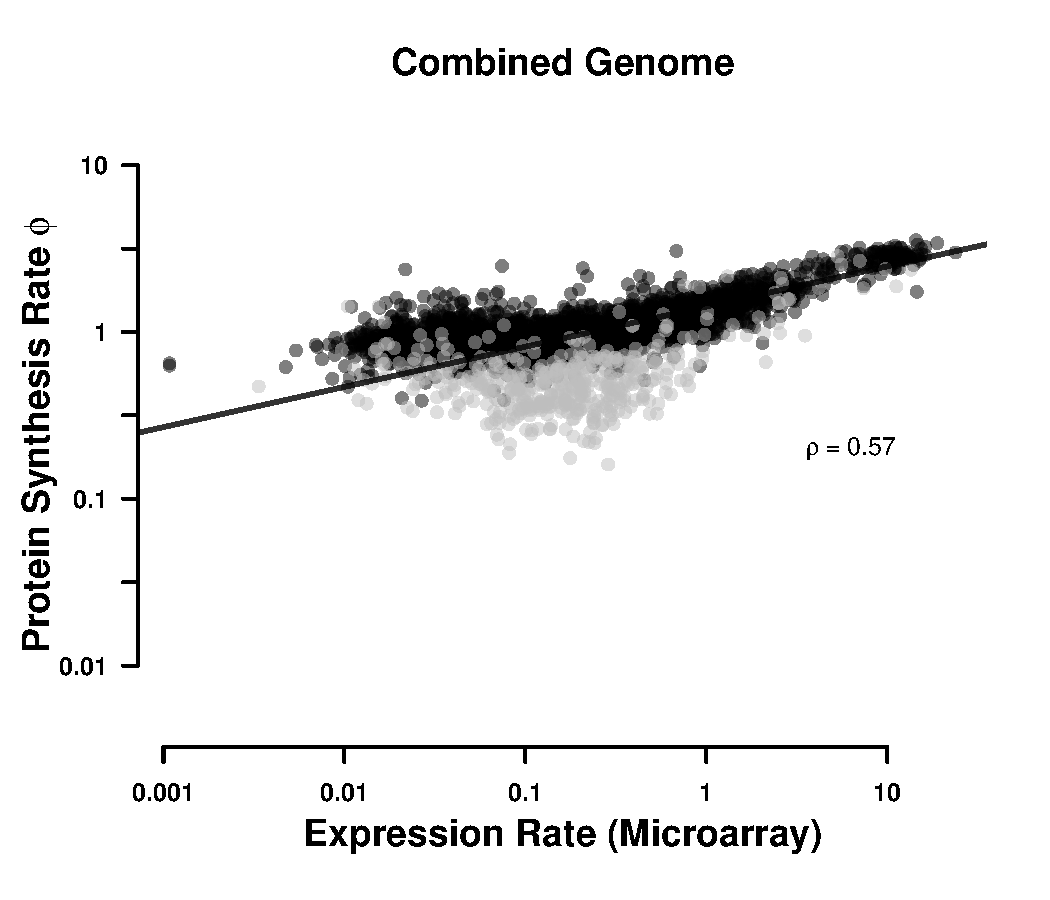
\includegraphics[width=.45\textwidth]{img/phi_corr_plot_whole_Genome_estim.pdf}
    \end{subfigure}
    \begin{subfigure}
        \centering
        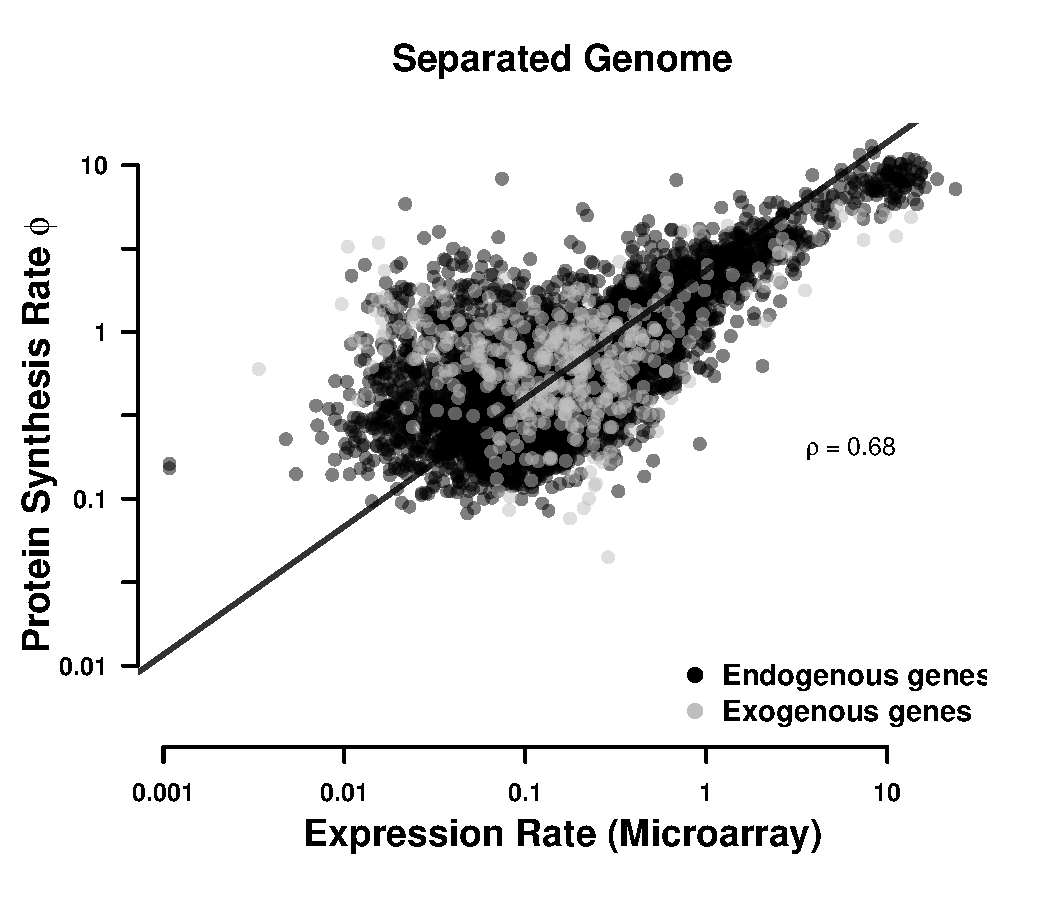
\includegraphics[width=.45\textwidth]{img/phi_corr_plot_split_Genome_estim.pdf}
    \end{subfigure}
    \caption{Person correlation of predicted protein synthesis rate $\phi$ with observed expression rate}
    \label{fig:phi_corr_two_cond}
\end{figure}

\begin{figure}[H]
    \centering
    \begin{subfigure}
        \centering
        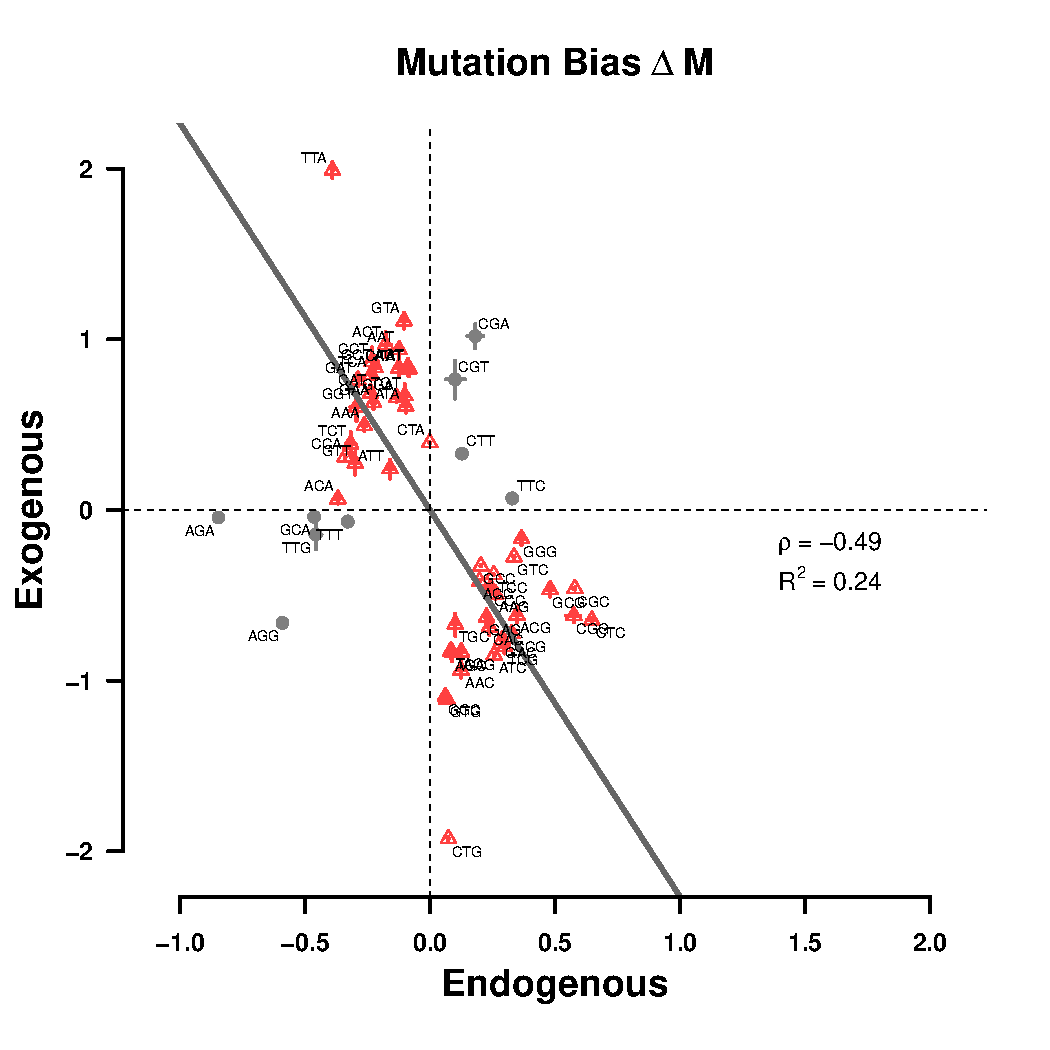
\includegraphics[width=.45\textwidth]{img/csp_corr_dm.pdf}
    \end{subfigure}
    \begin{subfigure}
        \centering
        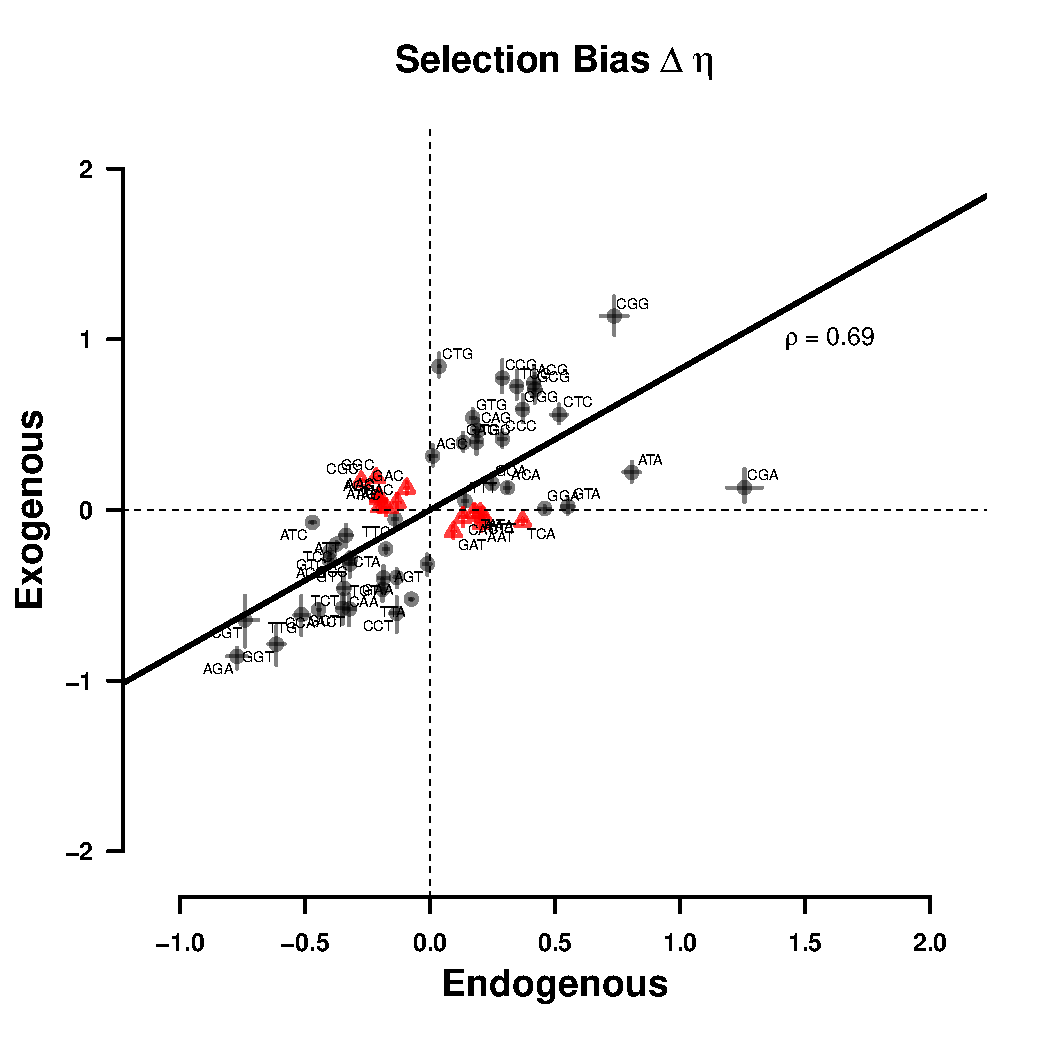
\includegraphics[width=.45\textwidth]{img/csp_corr_deta.pdf}
    \end{subfigure}
    \caption{Person correlation for CUB parameters estimated from endogenous and exogenous genes (red = opposite sign, black = same sign)}
    \label{fig:csp_comp}
\end{figure}

\begin{figure}[H]
     \centering
	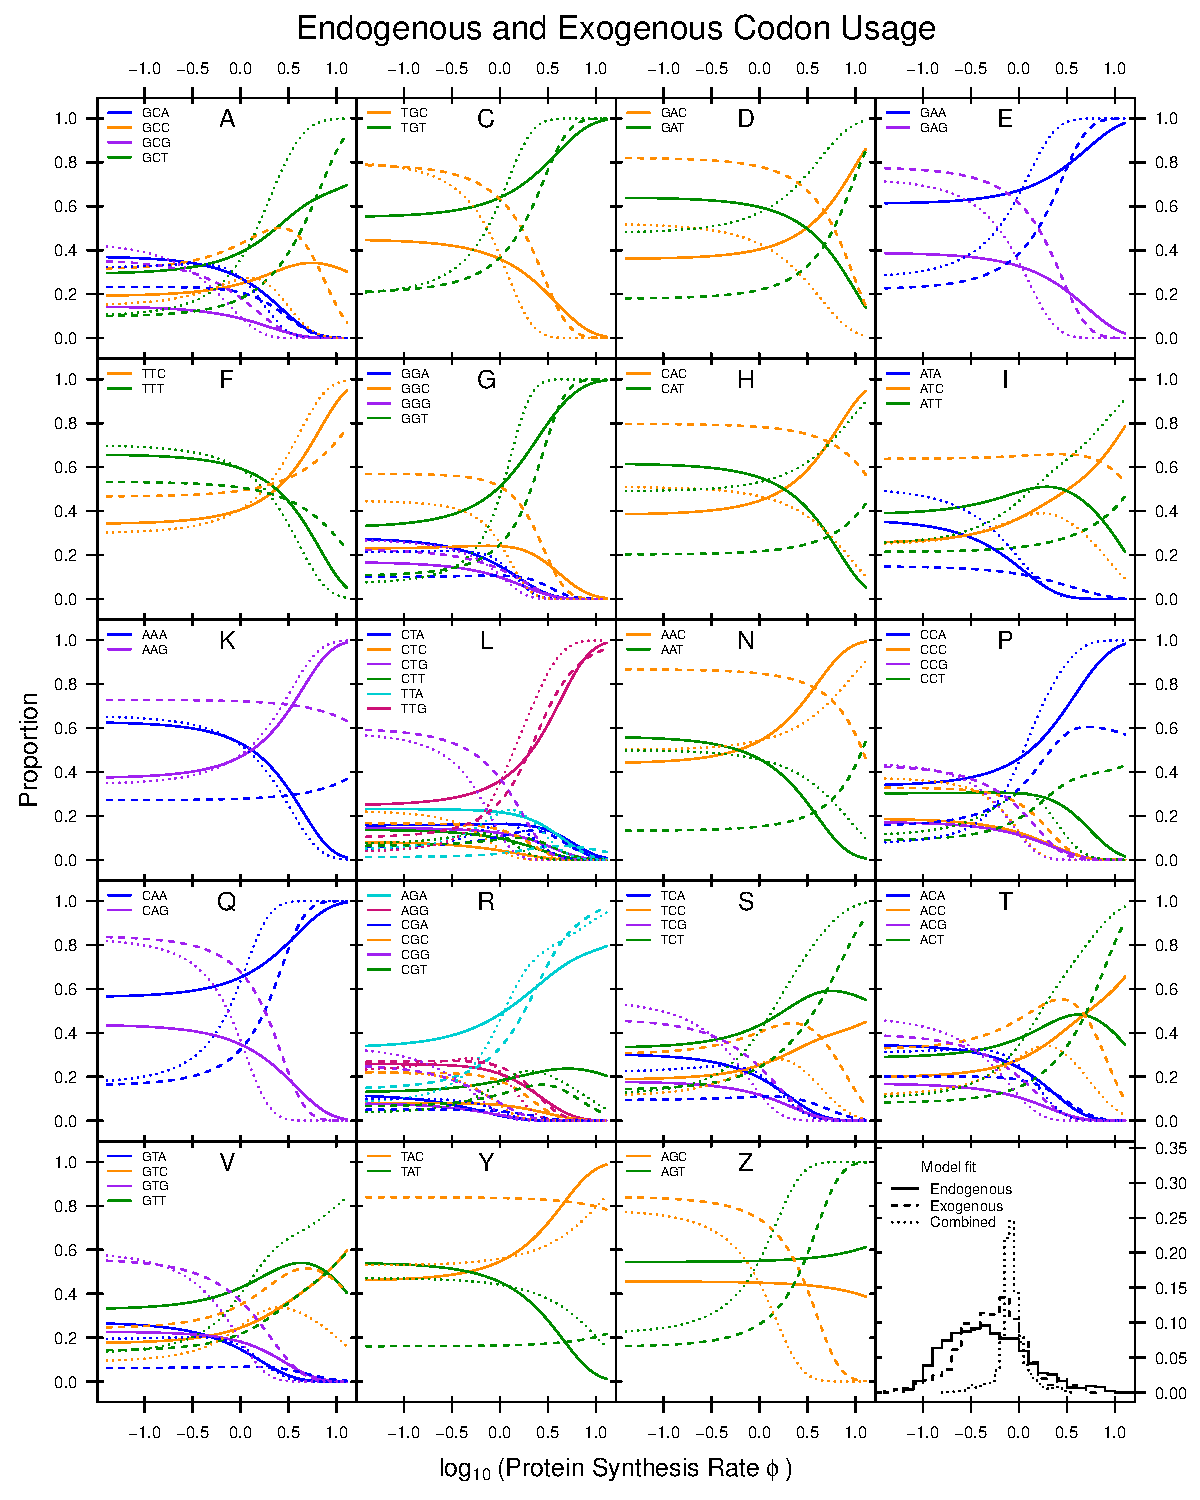
\includegraphics[width=\textwidth]{img/CUB_cleft_main.pdf}
	\caption{Codon Usage. Modify figure to indicate whether same AA is optimal in endogenous/exogenous region? }
	\label{fig:cub_all_aa}
\end{figure}

\begin{figure}[H]
     \centering
	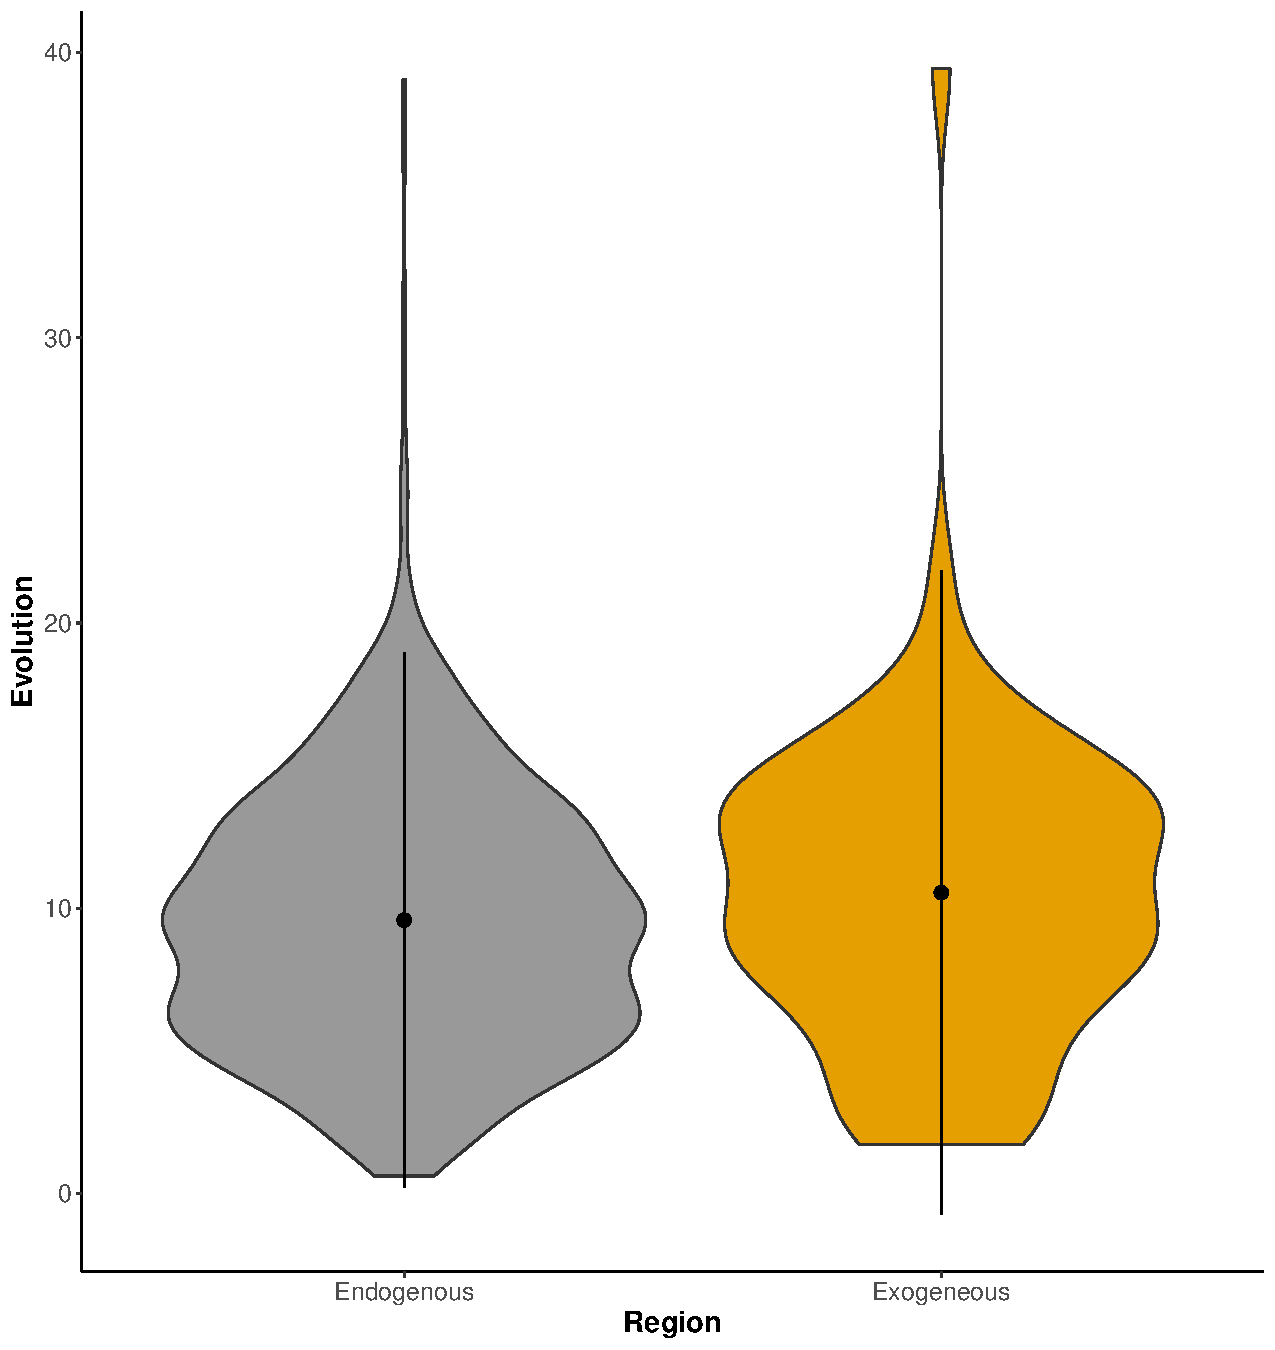
\includegraphics[width=\textwidth]{img/rate_of_evolution.pdf}
	\caption{Overall time passed along gene tree}
	\label{fig:rate_evol}
\end{figure}

\begin{figure}[H]
     \centering
	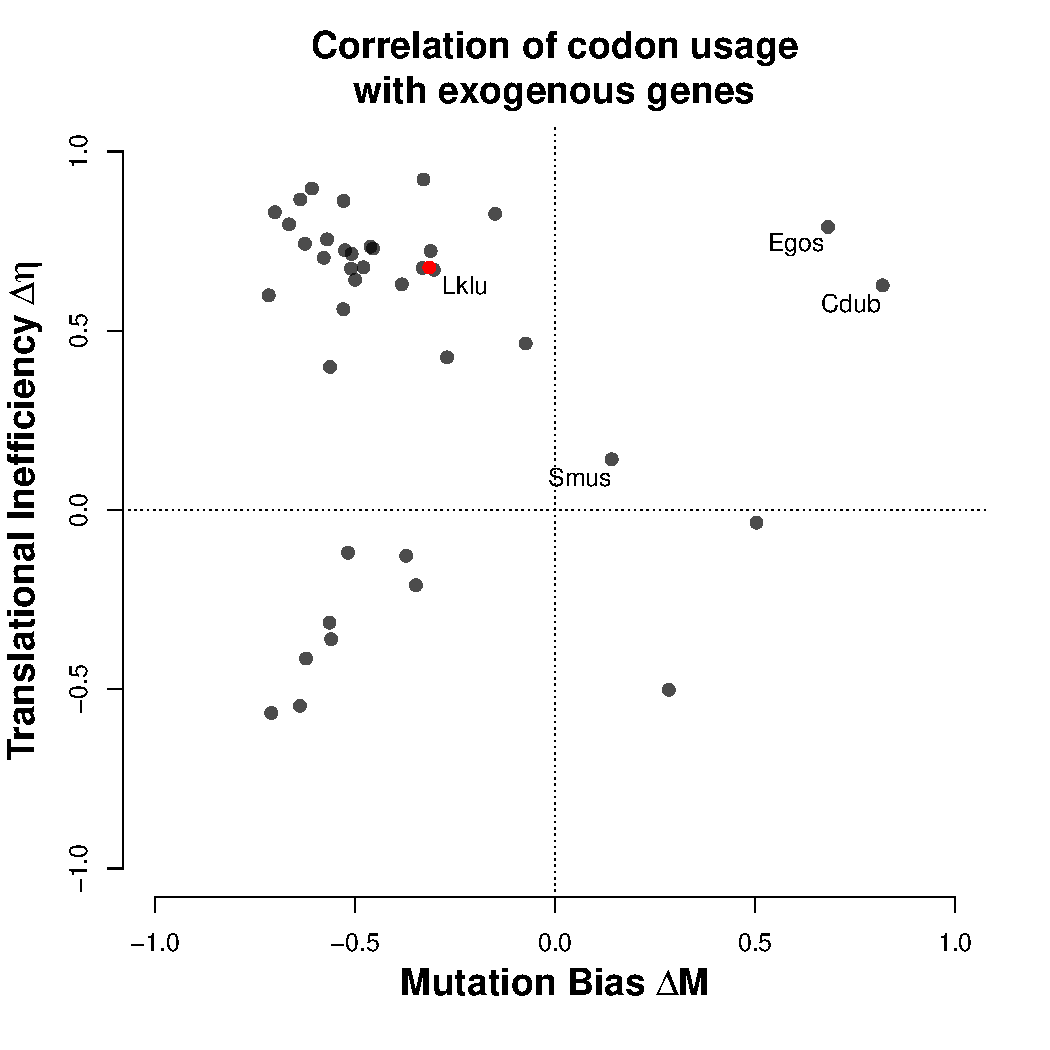
\includegraphics[width=\textwidth]{img/csp_correlations.pdf}
	\caption{Codon Usage}
	\label{fig:corr_all_species}
\end{figure}


\begin{figure}[H]
    \centering
    \begin{subfigure}
        \centering
        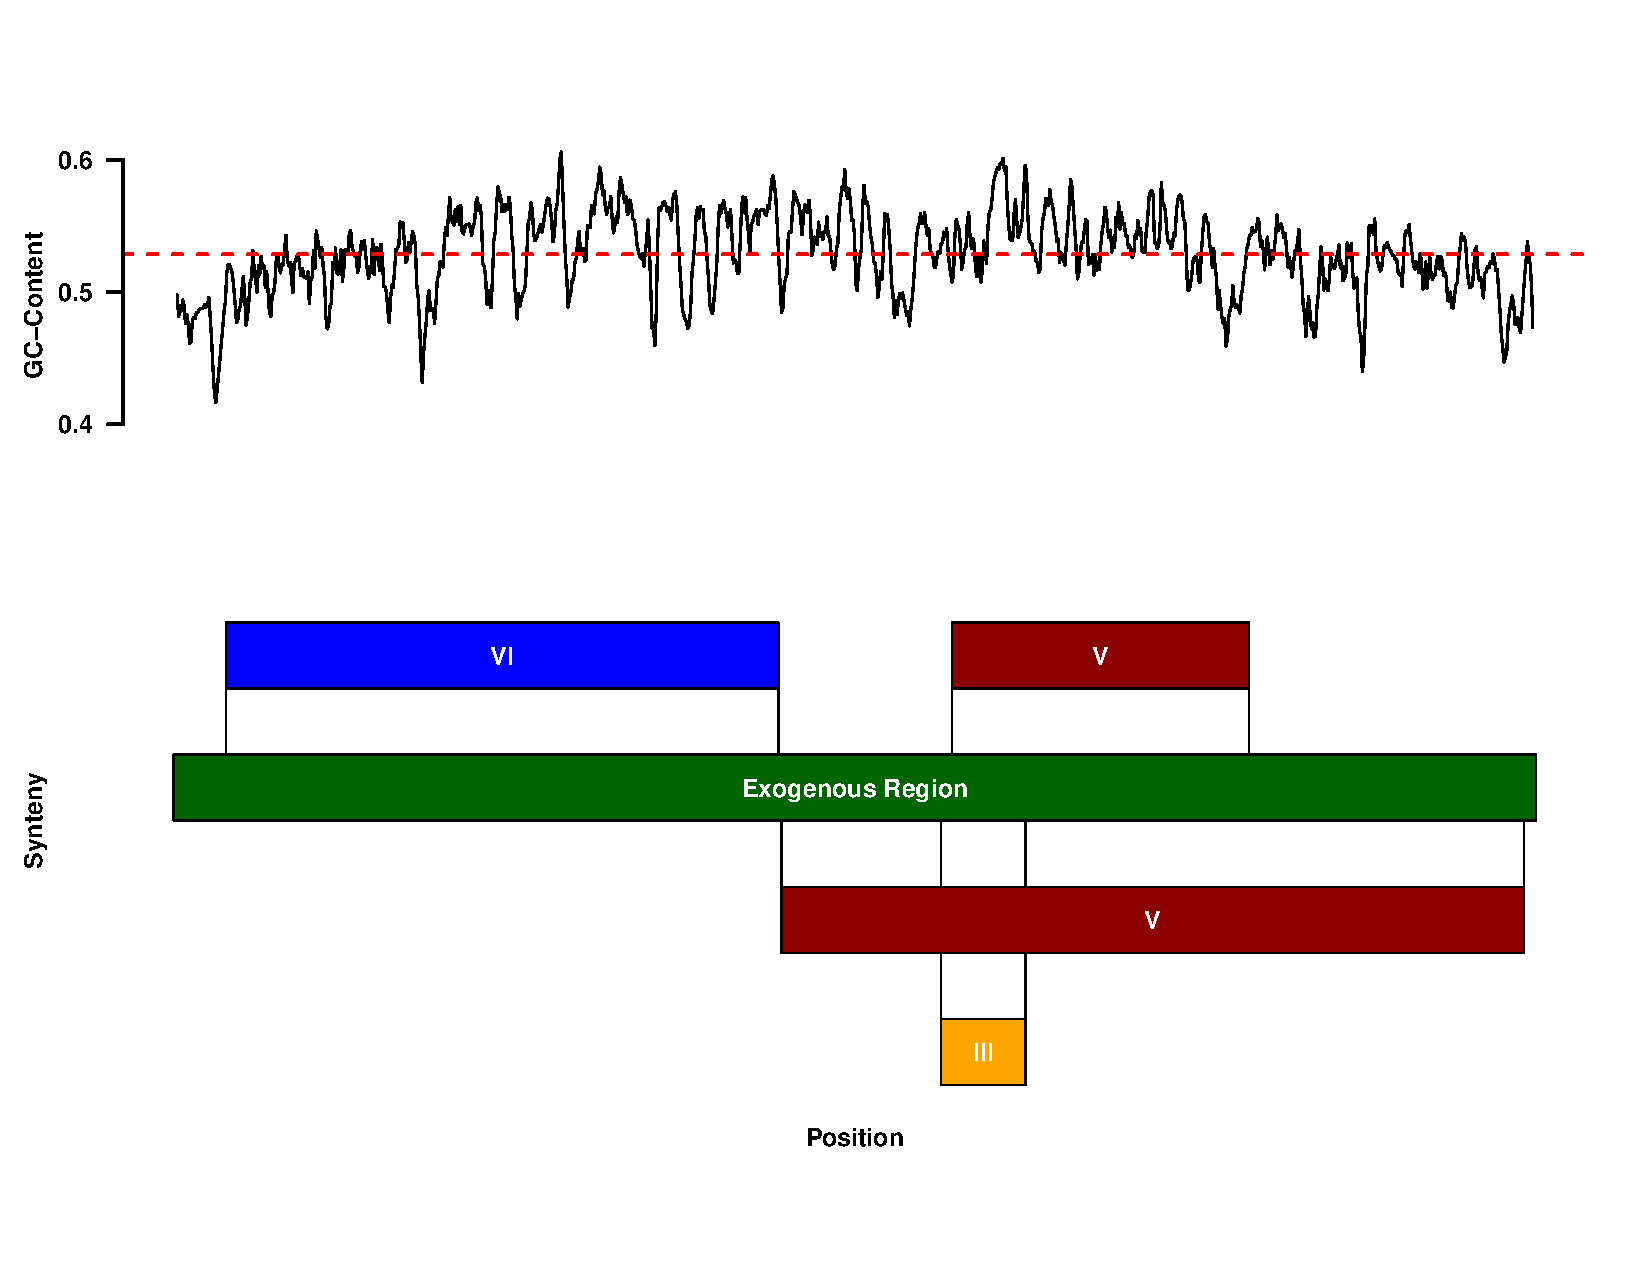
\includegraphics[width=.45\textwidth]{img/synteny_blocks_and_gc.pdf}
    \end{subfigure}
    \begin{subfigure}
        \centering
        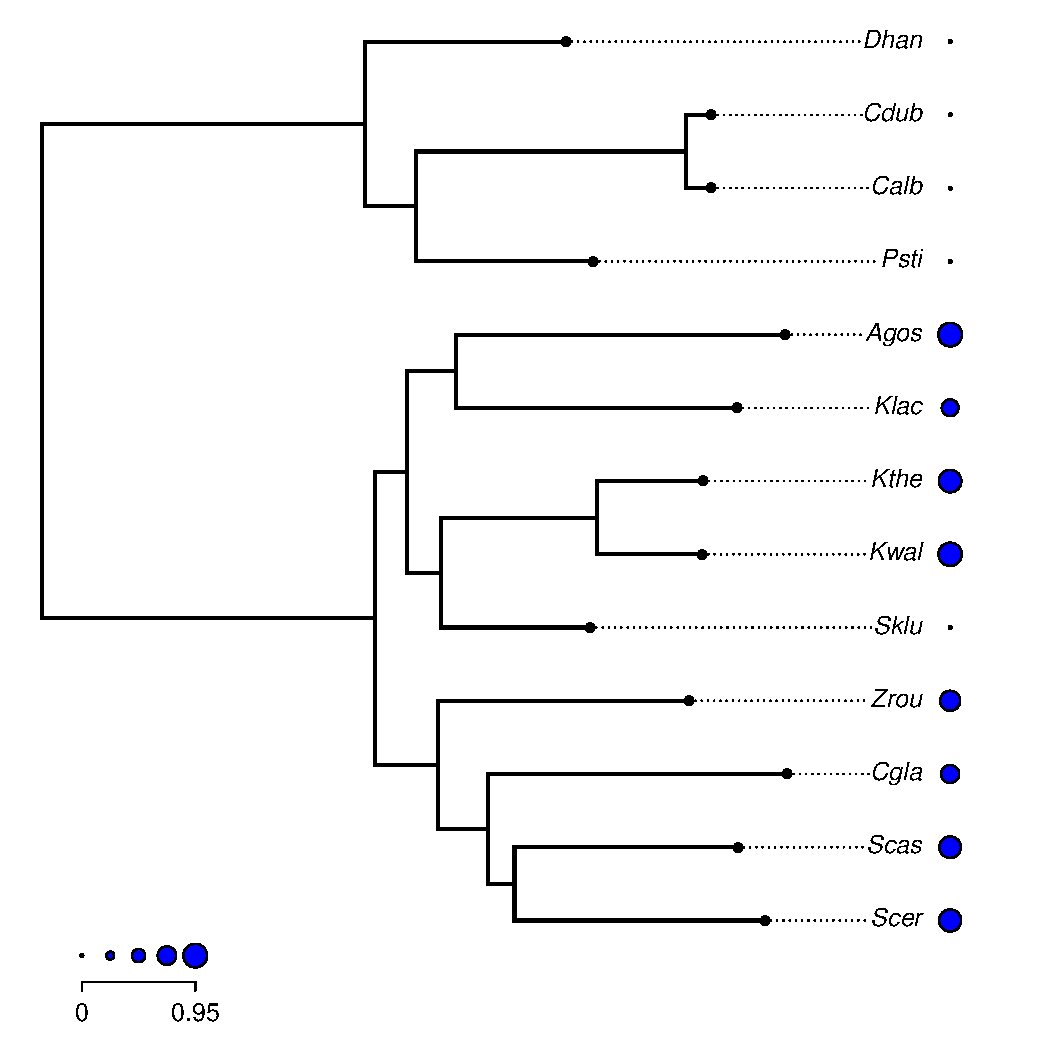
\includegraphics[width=.45\textwidth]{img/synteny_coverage.pdf}
    \end{subfigure}
    \caption{Synteny stuff}
    \label{fig:synteny_species}
\end{figure}


\begin{table}
\centering
\begin{tabular}{ | c | c | c | c | c | c | c | }
\hline
	Codon & Amino Acid & $\Delta M_{Egos}$ & $\Delta M_{Endo}$ & $\Delta M_{Exo}$ &$T_{Intro}$ & $T_{decay}$ \\ \hline
	TGC & Cys (C) & -3.28 & 0.20 & -1.34 & $4.81e8$ & $5.61e9$ \\ \hline
	GAC & Asp (D) & -2.57 & 0.58 & -1.26  & $2.88e8$ & $4.79e9$ \\ \hline
	GAA & Glu (E) & 2.47 & 0.45 & 1.26 & $6.30e8$ & $4.45e9$ \\ \hline
	TTC & Phe (F) & -1.46 & 0.66 & 0.14  & $1.19e8$ & $4.42e9$ \\ \hline
	CAC & His (H) & -2.31 & 0.48 & -1.37  & $2.41e8$ & $4.96e9$ \\ \hline
	AAA & Lys (K) & 0.96 & -0.53 & 0.99 & $-2.78e7$ & $6.67e9$ \\ \hline
	AAC & Asn (N) & -1.28 & 0.25 & -1.88 & $-2.54e8$ & $5.03e9$ \\ \hline
	CAA & Gln (Q) & 2.98 & -0.25 & 1.67 & $3.57e8$ & $6.68e9$ \\ \hline
	TAC & Tyr (Y) & -1.92 & 0.17 & -1.65 & $1.01e8$ & $5.43e9$ \\ \hline
	AGC & Ser$_2 $ (Z) & -3.11 & 0.18 & -1.68 & $3.10e8$ & $5.63e9$ \\ \hline
	& & & & & &   \\ \hline
	& & & & Mean: & $3.32e8$ ($4.5e8$) & $5.37e9$ ($5.25e9$) \\ \hline
	& & & & Std Error: & $1.24e8$ ($1.07e8$) & $8.10e8$ ($2.38e8$)\\ \hline
\end{tabular}
\caption{Mutation rate is $3.8e-10$ (Lang 2008), ignoring negative values in parenthesis. Decayed to $1 \%$. }
\label{tab:intro_age}
\end{table}


\end{document}








